% Proposed LaTeX figure environment for the PatternGrad conceptual diagram.
% Copy patterngrad_conceptual_diagram.pdf next to the manuscript (or adjust
% the path). Notation matches sn-article.tex (Eqs. ig_riemann, pg_kernel,
% pg_closed). The illustrated example is reproducible: LIN-WHITE, alpha=0.2,
% class y=0, test index 78 (first held-out evaluation sample).

\begin{figure}[t]
    \centering
    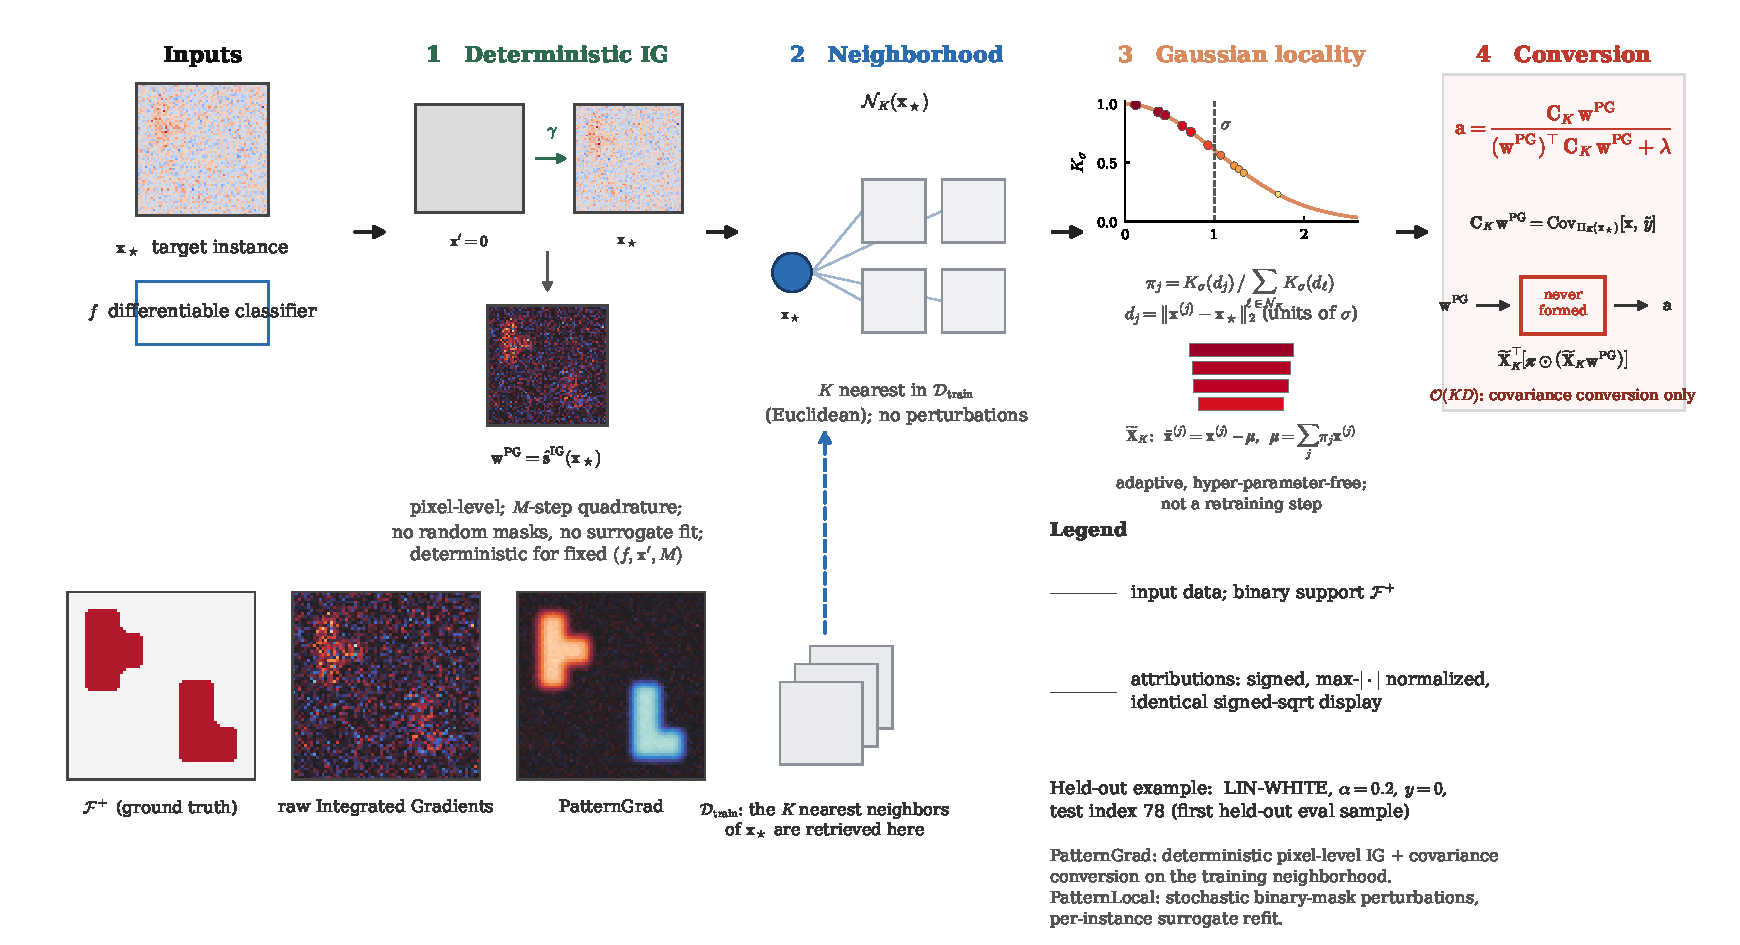
\includegraphics[width=\textwidth]{patterngrad_conceptual_diagram.pdf}
    \caption{The PatternGrad pipeline. Given a differentiable classifier $f$
    and a target instance $\mathbf{x}_\star$,
    \textcircled{\small 1}~a deterministic Integrated-Gradients surrogate
    $\mathbf{w}^{\mathrm{PG}} = \hat{\mathbf{s}}^{\mathrm{IG}}(\mathbf{x}_\star)$
    is computed at pixel level by $M$-step quadrature along the straight-line
    path from the zero baseline $\mathbf{x}' = \mathbf{0}$
    (Eq.~\eqref{eq:ig_riemann}); no stochastic perturbations or per-instance
    surrogate fitting are involved, and the only numerical error is the
    deterministic quadrature error of the $M$-step sum.
    \textcircled{\small 2}~The $K$ nearest training samples
    $\mathcal{N}_K(\mathbf{x}_\star)$ are retrieved from
    $\mathcal{D}_{\mathrm{train}}$ under the Euclidean metric, rather than
    synthesized as random perturbations or binary masks.
    \textcircled{\small 3}~A training-anchored Gaussian locality kernel
    assigns normalized weights $\pi_j = K_\sigma(d_j) /
    \sum_{\ell \in \mathcal{N}_K} K_\sigma(d_\ell)$ with
    $d_j = \|\mathbf{x}^{(j)} - \mathbf{x}_\star\|_2$ and the
    instance-adaptive bandwidth $\sigma = \operatorname{median}\{d_j\}$
    (Eq.~\eqref{eq:pg_kernel}); no bandwidth hyper-parameter is introduced,
    and no classifier retraining occurs. The weighted, centered neighborhood
    $\widetilde{\mathbf{X}}_K$ uses
    $\tilde{\mathbf{x}}^{(j)} = \mathbf{x}^{(j)} - \boldsymbol{\mu}$ with
    $\boldsymbol{\mu} = \sum_j \pi_j \mathbf{x}^{(j)}$.
    \textcircled{\small 4}~The surrogate response
    $\tilde{y} = (\mathbf{w}^{\mathrm{PG}})^\top \mathbf{x}$ is converted
    into the generative attribution pattern
    $\mathbf{a} = \mathbf{C}_K \mathbf{w}^{\mathrm{PG}} /
    ((\mathbf{w}^{\mathrm{PG}})^\top \mathbf{C}_K \mathbf{w}^{\mathrm{PG}} + \lambda)$
    (Eq.~\eqref{eq:pg_closed}), where
    $\mathbf{C}_K \mathbf{w}^{\mathrm{PG}} =
    \operatorname{Cov}_{\Pi_K(\mathbf{x}_\star)}[\mathbf{x}, \tilde{y}]$;
    the product is evaluated by the two-pass expression
    $\widetilde{\mathbf{X}}_K^\top[\boldsymbol{\pi} \odot
    (\widetilde{\mathbf{X}}_K \mathbf{w}^{\mathrm{PG}})]$ in
    $\mathcal{O}(KD)$ time and space, a cost of the covariance conversion
    step alone, without materializing $\mathbf{C}_K$.
    \emph{Bottom:} for one held-out LIN-WHITE test instance
    ($\alpha = 0.2$, $y = 0$, test index 78): the binary ground-truth
    support $\mathcal{F}^+$ (the union of the $\mathbf{a}^{\mathrm{T}}$ and
    $\mathbf{a}^{\mathrm{L}}$ regions, since the absence of one shape is as
    informative as the presence of the other), the raw Integrated-Gradients
    map, and the PatternGrad output. Attribution maps are signed and shown
    after identical max-magnitude normalization and a common signed-sqrt
    display transform; PatternGrad concentrates attribution on
    $\mathcal{F}^+$ while raw IG leaks into the background.}
    \label{fig:patterngrad_concept}
\end{figure}
